% Options for packages loaded elsewhere
\PassOptionsToPackage{unicode}{hyperref}
\PassOptionsToPackage{hyphens}{url}
%
\documentclass[
]{book}
\usepackage{amsmath,amssymb}
\usepackage{iftex}
\ifPDFTeX
  \usepackage[T1]{fontenc}
  \usepackage[utf8]{inputenc}
  \usepackage{textcomp} % provide euro and other symbols
\else % if luatex or xetex
  \usepackage{unicode-math} % this also loads fontspec
  \defaultfontfeatures{Scale=MatchLowercase}
  \defaultfontfeatures[\rmfamily]{Ligatures=TeX,Scale=1}
\fi
\usepackage{lmodern}
\ifPDFTeX\else
  % xetex/luatex font selection
\fi
% Use upquote if available, for straight quotes in verbatim environments
\IfFileExists{upquote.sty}{\usepackage{upquote}}{}
\IfFileExists{microtype.sty}{% use microtype if available
  \usepackage[]{microtype}
  \UseMicrotypeSet[protrusion]{basicmath} % disable protrusion for tt fonts
}{}
\makeatletter
\@ifundefined{KOMAClassName}{% if non-KOMA class
  \IfFileExists{parskip.sty}{%
    \usepackage{parskip}
  }{% else
    \setlength{\parindent}{0pt}
    \setlength{\parskip}{6pt plus 2pt minus 1pt}}
}{% if KOMA class
  \KOMAoptions{parskip=half}}
\makeatother
\usepackage{xcolor}
\usepackage{color}
\usepackage{fancyvrb}
\newcommand{\VerbBar}{|}
\newcommand{\VERB}{\Verb[commandchars=\\\{\}]}
\DefineVerbatimEnvironment{Highlighting}{Verbatim}{commandchars=\\\{\}}
% Add ',fontsize=\small' for more characters per line
\usepackage{framed}
\definecolor{shadecolor}{RGB}{248,248,248}
\newenvironment{Shaded}{\begin{snugshade}}{\end{snugshade}}
\newcommand{\AlertTok}[1]{\textcolor[rgb]{0.94,0.16,0.16}{#1}}
\newcommand{\AnnotationTok}[1]{\textcolor[rgb]{0.56,0.35,0.01}{\textbf{\textit{#1}}}}
\newcommand{\AttributeTok}[1]{\textcolor[rgb]{0.13,0.29,0.53}{#1}}
\newcommand{\BaseNTok}[1]{\textcolor[rgb]{0.00,0.00,0.81}{#1}}
\newcommand{\BuiltInTok}[1]{#1}
\newcommand{\CharTok}[1]{\textcolor[rgb]{0.31,0.60,0.02}{#1}}
\newcommand{\CommentTok}[1]{\textcolor[rgb]{0.56,0.35,0.01}{\textit{#1}}}
\newcommand{\CommentVarTok}[1]{\textcolor[rgb]{0.56,0.35,0.01}{\textbf{\textit{#1}}}}
\newcommand{\ConstantTok}[1]{\textcolor[rgb]{0.56,0.35,0.01}{#1}}
\newcommand{\ControlFlowTok}[1]{\textcolor[rgb]{0.13,0.29,0.53}{\textbf{#1}}}
\newcommand{\DataTypeTok}[1]{\textcolor[rgb]{0.13,0.29,0.53}{#1}}
\newcommand{\DecValTok}[1]{\textcolor[rgb]{0.00,0.00,0.81}{#1}}
\newcommand{\DocumentationTok}[1]{\textcolor[rgb]{0.56,0.35,0.01}{\textbf{\textit{#1}}}}
\newcommand{\ErrorTok}[1]{\textcolor[rgb]{0.64,0.00,0.00}{\textbf{#1}}}
\newcommand{\ExtensionTok}[1]{#1}
\newcommand{\FloatTok}[1]{\textcolor[rgb]{0.00,0.00,0.81}{#1}}
\newcommand{\FunctionTok}[1]{\textcolor[rgb]{0.13,0.29,0.53}{\textbf{#1}}}
\newcommand{\ImportTok}[1]{#1}
\newcommand{\InformationTok}[1]{\textcolor[rgb]{0.56,0.35,0.01}{\textbf{\textit{#1}}}}
\newcommand{\KeywordTok}[1]{\textcolor[rgb]{0.13,0.29,0.53}{\textbf{#1}}}
\newcommand{\NormalTok}[1]{#1}
\newcommand{\OperatorTok}[1]{\textcolor[rgb]{0.81,0.36,0.00}{\textbf{#1}}}
\newcommand{\OtherTok}[1]{\textcolor[rgb]{0.56,0.35,0.01}{#1}}
\newcommand{\PreprocessorTok}[1]{\textcolor[rgb]{0.56,0.35,0.01}{\textit{#1}}}
\newcommand{\RegionMarkerTok}[1]{#1}
\newcommand{\SpecialCharTok}[1]{\textcolor[rgb]{0.81,0.36,0.00}{\textbf{#1}}}
\newcommand{\SpecialStringTok}[1]{\textcolor[rgb]{0.31,0.60,0.02}{#1}}
\newcommand{\StringTok}[1]{\textcolor[rgb]{0.31,0.60,0.02}{#1}}
\newcommand{\VariableTok}[1]{\textcolor[rgb]{0.00,0.00,0.00}{#1}}
\newcommand{\VerbatimStringTok}[1]{\textcolor[rgb]{0.31,0.60,0.02}{#1}}
\newcommand{\WarningTok}[1]{\textcolor[rgb]{0.56,0.35,0.01}{\textbf{\textit{#1}}}}
\usepackage{longtable,booktabs,array}
\usepackage{calc} % for calculating minipage widths
% Correct order of tables after \paragraph or \subparagraph
\usepackage{etoolbox}
\makeatletter
\patchcmd\longtable{\par}{\if@noskipsec\mbox{}\fi\par}{}{}
\makeatother
% Allow footnotes in longtable head/foot
\IfFileExists{footnotehyper.sty}{\usepackage{footnotehyper}}{\usepackage{footnote}}
\makesavenoteenv{longtable}
\usepackage{graphicx}
\makeatletter
\def\maxwidth{\ifdim\Gin@nat@width>\linewidth\linewidth\else\Gin@nat@width\fi}
\def\maxheight{\ifdim\Gin@nat@height>\textheight\textheight\else\Gin@nat@height\fi}
\makeatother
% Scale images if necessary, so that they will not overflow the page
% margins by default, and it is still possible to overwrite the defaults
% using explicit options in \includegraphics[width, height, ...]{}
\setkeys{Gin}{width=\maxwidth,height=\maxheight,keepaspectratio}
% Set default figure placement to htbp
\makeatletter
\def\fps@figure{htbp}
\makeatother
\setlength{\emergencystretch}{3em} % prevent overfull lines
\providecommand{\tightlist}{%
  \setlength{\itemsep}{0pt}\setlength{\parskip}{0pt}}
\setcounter{secnumdepth}{5}
\usepackage{booktabs}
\ifLuaTeX
  \usepackage{selnolig}  % disable illegal ligatures
\fi
\usepackage[]{natbib}
\bibliographystyle{plainnat}
\IfFileExists{bookmark.sty}{\usepackage{bookmark}}{\usepackage{hyperref}}
\IfFileExists{xurl.sty}{\usepackage{xurl}}{} % add URL line breaks if available
\urlstyle{same}
\hypersetup{
  pdftitle={Regresi Untuk Penelitian},
  pdfauthor={andri Faisal},
  hidelinks,
  pdfcreator={LaTeX via pandoc}}

\title{Regresi Untuk Penelitian}
\author{andri Faisal}
\date{2025-01-24}

\usepackage{amsthm}
\newtheorem{theorem}{Theorem}[chapter]
\newtheorem{lemma}{Lemma}[chapter]
\newtheorem{corollary}{Corollary}[chapter]
\newtheorem{proposition}{Proposition}[chapter]
\newtheorem{conjecture}{Conjecture}[chapter]
\theoremstyle{definition}
\newtheorem{definition}{Definition}[chapter]
\theoremstyle{definition}
\newtheorem{example}{Example}[chapter]
\theoremstyle{definition}
\newtheorem{exercise}{Exercise}[chapter]
\theoremstyle{definition}
\newtheorem{hypothesis}{Hypothesis}[chapter]
\theoremstyle{remark}
\newtheorem*{remark}{Remark}
\newtheorem*{solution}{Solution}
\begin{document}
\maketitle

{
\setcounter{tocdepth}{1}
\tableofcontents
}
\hypertarget{about}{%
\chapter{About}\label{about}}

This is a \emph{sample} book written in \textbf{Markdown}. You can use anything that Pandoc's Markdown supports; for example, a math equation \(a^2 + b^2 = c^2\).

\hypertarget{usage}{%
\section{Usage}\label{usage}}

Each \textbf{bookdown} chapter is an .Rmd file, and each .Rmd file can contain one (and only one) chapter. A chapter \emph{must} start with a first-level heading: \texttt{\#\ A\ good\ chapter}, and can contain one (and only one) first-level heading.

Use second-level and higher headings within chapters like: \texttt{\#\#\ A\ short\ section} or \texttt{\#\#\#\ An\ even\ shorter\ section}.

The \texttt{index.Rmd} file is required, and is also your first book chapter. It will be the homepage when you render the book.

\hypertarget{render-book}{%
\section{Render book}\label{render-book}}

You can render the HTML version of this example book without changing anything:

\begin{enumerate}
\def\labelenumi{\arabic{enumi}.}
\item
  Find the \textbf{Build} pane in the RStudio IDE, and
\item
  Click on \textbf{Build Book}, then select your output format, or select ``All formats'' if you'd like to use multiple formats from the same book source files.
\end{enumerate}

Or build the book from the R console:

\begin{Shaded}
\begin{Highlighting}[]
\NormalTok{bookdown}\SpecialCharTok{::}\FunctionTok{render\_book}\NormalTok{()}
\end{Highlighting}
\end{Shaded}

To render this example to PDF as a \texttt{bookdown::pdf\_book}, you'll need to install XeLaTeX. You are recommended to install TinyTeX (which includes XeLaTeX): \url{https://yihui.org/tinytex/}.

\hypertarget{preview-book}{%
\section{Preview book}\label{preview-book}}

As you work, you may start a local server to live preview this HTML book. This preview will update as you edit the book when you save individual .Rmd files. You can start the server in a work session by using the RStudio add-in ``Preview book'', or from the R console:

\begin{Shaded}
\begin{Highlighting}[]
\NormalTok{bookdown}\SpecialCharTok{::}\FunctionTok{serve\_book}\NormalTok{()}
\end{Highlighting}
\end{Shaded}

\hypertarget{pendahuluan}{%
\chapter{Pendahuluan}\label{pendahuluan}}

Dalam waktu penelitian kita membutuhakan hal sesuatua yang menyeelsaikan permasalahan kita. Manusia mempunyai naluri untuk menyelesaikan masalah sendiri. Dahulu banyak sekali hal yang bisa kita carikan. Hal mencari soulusi yang akan ada untuk mencari yang memudahkan hidup mereka sendiri.
Ada hal yang selalu berubah itu kita tidak pungkisiri seperti itu. Kita kesulitan untuk memprediksi suatua atau beberapa hal. Dalam regresi kita akan melihat hubungan antara satu dengan variabel yang lainnya . Kita bisa memprediksi satu variabel tersebut dengan caa melihat variabel yang lain.
Sifat asli manusia yang mempunyai rasa ingin tahu dan mencari faktor yang menjadi pneghubung. Kenapa sesuatua yaitu faktor independen mempunyai pengaruh. Ada beberapa pengaruh yang harus di cari untuk menerangkan hal yang lain.
Dalam buku ini saya akan menyajikan pengenalan terhadap regresi itu sendiri. \emph{Regresi adalah sesuatu metode perhitungan atau kalkulasi dari covarian berhubungan antara variabel bebas dan juga variabel tak bebas.} Dari nilai ini kita akan dapat menduga nilai hubungan yang erat yang diwakili dengan nilai satu sampai dengan nilai 0. Sesudah itu akan diterangkan konsep dasar statistik mengenai regresi. Kita tahu regresi adalah berbeda dnegan stataistik sebelumnya yakni stataistik deskriptif. Untuk kalkukasi regresi termasuk da;lam stataistik analisis. Dari sini seorang mulai menganalisis data yang sudah ada berita megenai hubungan antara kedua data.
Sebelumnya juga ada suatau ulangan mengenai apa itu stataistik. Pengenalan regresi akan ada pada variabel. Variabel yang merupakan nilai dari kharakteristik suatu sample. Kita mendapat nilai tersebut untuk dihubungkan dengan dengan yang lain. Penulis memandang penting agar para pembaca bisa untuk memahami maksuda dari model analisis regresi tersebut.
Setelah penegnalan maka masuk ke dalam regresi sederhana yang hanya memuat satu variabel independen saja. Dalam regresi sederhana , maka faktor dependen atau variabel terikat hanya terpengaruh dari satu variabel saja. Ada variabel dominan yang dapat mempengaruhi suatu faktor seperti hubungan anatara penghasilan dengan kepandaian. Bisa jadi nilai kepandaian atau variabel kepandaian tersebut dapat ubtu mempengaruhi penghasilan orang.
Karena hanya satu variable maka rasanya kurang untuk menghitung hanya satu variabel saja arenanya ada regresi dengan eberapa faktor independen. Faktor-faktor inilah yang diduga dengan bersama-sama turut dalam memepgaruhi variabel indeonden tersbeut. Dengan regresi yang begitu komplek tersebut maka akan ada sejumlah asumsi.
Sebelum ke asumsi namanya regresi juga mempunyai syarat yang harus dipenuhi. Appaun model analisis juga harus memenuhi syarat. Dari syarat tersebut nanti kita akan mendapatkan sutaua bentuk peramalan yang sesuai atau sedikit kesalahan. Peramalan yang baik adalah peramalan yang bukan memiliki kesalahalan akan tetapi peramalan yang baik adalah yang kesalahannya sedikit. Dengan adanya asusmi linear itu akan memastikan kalau model sudah cukup untuk memenuhi kriteria peramalan yang baik.
Adapun asumsi linear yang harus dipenuhi seperti multikolinearitas, autokorelasi, heteroskedatisitas dan lainnya. Dalam regresi linear juga harus mempertimbangkan asumsi normal. Data harus terdistribusi normal agar setiap bentuk pendugaan akan benar.
Setelah regresi selesai maka ada evaluasi model dengan ebebrapa kriteria seperti nilai MSE dan MAE. Dengan penulaian seperti ini kita akan mengetahu ada regresi yang baik. Buku ini ditutup dengan studi kasus agar setiap pembavca dapat mempelajari kasus apa yang terjadi. Hal ini akan bisa untuk semakin mendalami maksud dari pelajaran regresi kali ini.

\hypertarget{regresi-linier-sederhana}{%
\chapter{Regresi Linier Sederhana}\label{regresi-linier-sederhana}}

Regresi Linear Sederhana

Grafik Pencar atau Scatter Graph
Salah satu hal yang penting adalah ketika kita mau menduga hubungan antara variabel X dengan variabel Y yakni dengan scatter graph. Dengan gambar yang ada hubungan. Variabel Y akan kita tempatkan di bagian vertikal atau bagian yang menghadap ke atas sebaliknya dengan bagian X yang mendatar seperti horizontal.

Kita memasangkan sesuai dengan pasangan nilai data tersebut X dan Y. Jangan pasang teracak agar kita bisa melihat hubungan antara keduanya. Pasangan data tersebut adalah yang termasuk dalam individu misalnya ada seorang yang mempunyai pendapatan X dengan pengeluaran Y maka nilai itu yang kita pasangkan bukan malah membuat pendapatan seorang tertentu dengan pengeluaran yang lain karena itu akan menjadi berbeda nilainya.
Dari hubungan tersebut akan membentuk scatter graph. Ada sejumlah titik-titik yang menyebar atau mengumpul di sekitar grafik pencar scatter graph tersebut. Titik titik itu mewakili banyak individu yang memiliki nilai dari kedua variabel X dan Y.
Banyaknya kumpulan titik atau scatter itu bergantung dari banyaknya daat tersebut. Semakin banyak jumlah data yang dibuat sampel adalah dengan dimasukkan dalam grafik tersebut. Ada beberapa hal yang dapat kita pelajari dari scatter plot seperti:
1. Pola dari titik tersebut mempunyai pola seperti cenderung mengumpul di satu tempat karena nilanya mempunyai yang sama
2. Trend. Kita dapat melihat suatu trend ketika ada satu garis yang bisa kita tarik pada titik tersebut dan kita menunjukkan ada yang bisa menunjukan garis ke atas atau bahkan tidak memiliki trend.
3. Outlier. Outlier adalah nilai yang terpencil . Ia hanya sendiri dan jauh di pinggir atau ditengah nilai-nilai yang lain karenanya disebut outlier. Outlier tentu sedikit dan ini menyebabkan data tidak normal.

Regresi Linear adalah salah satu cara untuk melihat hubungan antara variabel bebas dengan variabel tidak bebas. Dalam hal ini yang mempengaruhi adalah variabel yang bebas sedangkan yang dipengaruhi adalah variabel tidak bebas. Dalam regresi hanya mengenal satu arah saja pengaruh yakni variabel bebas terhadap variabel dependen dan bukan sebaliknya.
Pembatasan itu dengan tegas agar dalam mencari hubungan tidak akan ada kekeliruan. Misalnya pengaruh garam terhadap darah tinggi maka dari sini kita akan mencari hubungan antara garam dengan darah tinggi. Garamlah yang mempengaruhi tingginya tekanan darah (tensi) seseorang. Dengan alasan ilmiah dan penjelasan kalau zat garam akan meningkatkan tekanan darah tersebut. Kita tentu tidak akan menempatkan garam sebagai hal yang dependen tetapi ia adalah sesuatau yang bebas dalam hal ini karenanya ia mempengaruhi tekanan darah tinggi. Apakah ia akan menjadi faktor yang dipengaruhi. Hal itu bisa saja kalau dalam konteks yang lain misalnya kalau garam itu akan dipengaruhi oleh jumlah sinar matahari yang menerpa bumi.
Regresi linear pertama kali dikenalkan oleh Galton yang menemukan adanya hubungan tinggi anak dengan tinggi orang tuanya. Ia menghitung jumlah banyaknya anak yang mempunyai dengan tinggi orang tuanya. Hal ini berkaiatan dengann keturunan atau hereditas. Galton ingin menemukan apakah ada tinggi orang tua akan mempengaruhi tinggi sang anak.\\
Regresi linear hanya memeriksa antara hubungan variabel beas dengan variabel tidak bebas. Dalam regresi ini karena hanya ada satu maka disebut juga regresi linier sederhana (simple linear regression). Metode seperti ini dipakai seperti di ilmu bisnis, ekonomi, manajemen, komunikasi dan ilmu sosial lainnya.
Dalam regresi sederhana kita akan menggambarkan hubungan dengan garis y= a+ bx. Persamaan ini dihasilkan dari perhitungan regresi terhadap dua variabel tersbeut. Untuk nilai b diperoleh dengan perhitungan jelaskan dulu mengenai perhitungan ada simpangan x dengan simpangan y dibagi dengan jumlah sample atau n.~maka bisa dilihat seperti ini. Kemudian nilai a diperoleh dari nilai y rata-rata dikurangi b dikalikan dengan nilai rata-rata X dan akan kita peroleh nilai a tersebut. Bisa saja dengan menggunakan nilai perhitungan komputasi seperti Excel atau menggunakan software statistic lainnya.
Dimana a = nilai intercept atau nilai konstanta
b = koefisen slope atau kemiringan
Nilai a adalah konstanta ini adalah nilai awal dari persamaan suatu garis persamaan regresi tersebut. Nilai ini selalu ada. Hal yang ketika terjadi nilai regresor tersebut nol maka tetap saja nilai untuk Y prediksi tetap ada. Inilah nilai yang dinamakan nilai konstanta. Terkadang nama konstanta atau alpha disebut juga intercept sedangkan Beta dinamakan juga slope parameter atau ada juga yang menamakannya parameter.
Y (x=0) = a + bx
Y = a + 0.x = a
Nilai b ini menunjukkan kemiringan dari garis yang menunjukan hubungan antara y dengan X nilai positif berarti nilai yang menunjukkan seiringan atau hubungan yang sama-sama naik atau sama-sama turun. Ketika variabel independen mempunyai nilai yang positif maka akan merubah juga variabel dependen juga akan turut berubah menjadi positif. Bagaimana kalau nilai alpha menjadi 0 maka nilai persamaan tersebut akan memotong garis x karena tidak ada nilai alphanya.
Pengaruh nilai independen bergantung dengan koefisein semakin besar maka satau perubahan akan menjadi lebih besar dengan kemiringan yang curam sekali. Misalnya Y = 0,1 + 10 X berarti pengganda dari nilai regresi tersebut akan semakin besar dengan nilai tersebut. Jika nilai kurang dari 1 namun masih nilai positif maka kemiringan tetap ke sebelah kanan jadi nilai X meningkat namun dengan peningkatan nilai tersebut semakin kecil bukan besar. Untuk nilai yang negatif menunjukkan nilai tersebut adalah saling bertolak belakang. Ketika variabel independen bergerak naik maka yang terjadi adalah variabel dependen akan menurun dan sebaliknya. Hubungan yang negatif berarti juga saling bertolak belakang dan penambahan variabel independen akan mengurangi variabel dependen tersebut.

\hypertarget{keterbatasan-regresi-linear}{%
\section{Keterbatasan Regresi Linear}\label{keterbatasan-regresi-linear}}

Metode regresi linear adalah metode yang mendapatkan cara untuk menyelidiki hubungan antara variabel dependen dengan variabel independen. Dengan regresi tersebut kita akan mendapatkan nilai korelasi dari persamaan tersebut. Dari dua data yang disamakan tersebut kita akan mendapatkan suatu persamaan r yang mempunyai nilai -1≤r≤1 dengan perincian terhadap berikut.

Nilai R Arti
0,00 - 1,99 Sangat Lemah
2,00 - 3,99 Lemah
4,00 -- 5,99 Sedang
6,00 -- 7,99 Kuat
8,00 -1,00 Sangat Kuat

Perbedaan nilai R2 dengan koefisien
Kalau koefisien menyebutkan nilai koefisen menunjukkan banyaknya atau kuatnya nilai regresi tapi hati-hati kalau hal tersebut adalah berhubungan dengan nilai r dengan nilai koefisen regresi. Baik r dan beta adalah koefisien kalau beta adalah koefisien regresi sedangkan nilai r adalah koefisein korelasi. Koefisien regresi adalah menunjukkan besarnya hubungan ada suatu hubungan yang menjadi pengganda (multiplier). Koefisien regresi juga menjadi unsur dalam persamaan regresi. Hubungan ini menunjukkan akan ada besarnya pengali saja. Sedangkan koefisen korelasi adalah nilai yang menunjukkan adanya seberapa erat hubungan tersebut.
Nilai koefisein regresi menaksir atau meramal nilai Y terhadap nilai X, sedangkan kalau untuk nilai R tersebut memperkirakan keeratan hubungan. Apakah nilai tersebut mempunyai keeratan dari nilai r tersebut. Nilai dalam korelasi r dapat disimpulkan apakah ada hubungan yang kuat atau sama sekali tidak ada hubungan dalam kedua variabel tersebut. Sedangkan untuk nilai koefisein regresi maka kita akan melihat lebih jauh lagi untuk mengintrepretasikan nilai tersebut. Kita dapat menyimpulkan karena nilai dari data mentah antara variabel X dengan Y sudah berbeda. Karena nilai X dan Y mempunyai perbedaan yang besar sehingga nilai koefisiennya menjadi besar. Setiap pengaruh nilai satu independent maka akan berdampak besarnya sesuai dengan koefisen yang dihasilkan.

Kertebatasan
Sebagai model awal yang menunjukkan hubungan anatara variabel indpenden dan variable dependen ilmu ini adalah atau metode yang memberikan suatu pengetahunan dalam mencari hubungan tersebut. Ada beberpa variabel yang sebelumnya belum diketahui dan mungkin hanya estimasi tersbeut.
Perhitungan tersebut menghasilkan suatu hubungan yang merata ataupun hubungan seberapa besar pengaruh atau pengganda tersebut dalam koefisien regresi.

\hypertarget{regresi-linear-dengan-kategori}{%
\section{Regresi linear dengan kategori}\label{regresi-linear-dengan-kategori}}

Bagaimana kita bisa melakukan regresi linear dengan data kategori atau variabel independennya adalah variabel bebas. Hal itu bisa saja. Kalau kita menganggap ada perbedaan antara nilai mahasiswa dan mahasiswi maka kita akan bisa melihat perbedaan keduanya, misalnya Y=a + bx pada saat nilai untuk perempuan maka nilanya adalah alpha saja sedangkan pada saat pria ada nilai alpha plus beta.
Untuk melakukan regresi kita bisa melakukan hal itu dengan hati-hati. Kedua regresi ini akan menujukkan dua perbedaan karena adanya variable dikotomi tersebut. Untuk membedakan variable mana yang satu dan mana yang nol berdasarkan kebiasaaan saja. Misalnya kebiasaan dari dalam memilih sebuah regresi kategori untuk nilai nol (0) adalah dengan jenis kelamin perempuan dan juga maka akan ada yang dapat nilai satu (1) untuk nilai untuk laki-laki.
Adapun regresi dengan nilai kategori karena terjadinya perbedaan yang cukup kentara atau signfikan dari kedua kategori tersebut. Di negeri belahan Timur seperti Indonesia, kita tahu ada suatu diskriminasi upah antara pria dan wanita. Pria lebih menerima banyak upah karena hasil pekerjaan mereka lebih banyak dari para wanita.
Ketika ada dua hubungan yang berbeda ini maka akan dapat menjadikan nilai persamaan regresi bisa saja menjadi bias.

\hypertarget{latihan}{%
\section*{Latihan}\label{latihan}}
\addcontentsline{toc}{section}{Latihan}

Jawabalah pertanyaan dengan kata yang tepat

\begin{enumerate}
\def\labelenumi{\arabic{enumi}.}
\item
  Jelaskan Konsep regresi linear menurut anda?
\item
  Apa maksud Koefisen Korelasi tersebut?
\item
  Apakah wajib dalam menjelaskan regresi menggunakan diagram Scatter?
\item
  Anda mendapatkan pengetahuan variable bebas A dan variable tidak bebas B , bagaimana anda menenutukan garis regresi linear yang terbaik
\item
  Pada setiap regresi ada residual atau sisa? Jelaskan apa maksud resisdual positif dan residual negative?
\item
  Hasil output menunjukkan jika persamaan regresi adalah y=3x +5 apa arti dari persamaan regresi diatas?
\item
  Dalam regresi ada namanya prediksi dan estimasi . apa perbedaan dari keduanya?
\item
  Apakah heteroskedatisitas digunakan dalam regresi linier sederhana? Jelaskan?
\item
  Jelaskan bagaimana variable independent dapat menjelaskan variable dependen?
\item
  Jika nilai R square sekitar 0,90. Apakah artinya itu?
\end{enumerate}

\hypertarget{regresi-linier-berganda}{%
\chapter{Regresi Linier Berganda}\label{regresi-linier-berganda}}

Suatu faktor bukan dipengaruhi satu faktor saja. Seorang yang sukses bukan berasal dari ayah atau ibu yang sukses saja karena ada faktor lain. Ada anak orang kaya yang menjadi miskin karena tidak bisa mengelola harta ayahnya saja. Pada anak yang miskin ia bisa mendapatkan pendidikan dan ia meraih kekayaan yang melimpah karena keahliannya. Dalam praktik regresi linier sederhana sulit sekali dipraktekkan dan pencarian nilai tersebut hanya sederhana untuk mencari faktor yang dapat mempengaruhi faktor independen lainnya.

Adanya regresi berganda karena keterbatasan regresi linear itu maksudnya yang sederhana karena tidak mungkin bahwa hal yang mempengaruhi tersebut hanya satu faktor. Sangat sederhana kalau suatu peubah dipengaruhi oleh beberapa peubah yang lainnya.

Kita bisa melihat kalau nilai r square itu begitu rendah sekali karena pengaruhnya sedikit sekali. Maka kita harus mencari peubah lain yang akan mempengaruhi juga dan akan meningkatkan nilai R kuadrat. Memang tidak ada jaminan kalau peningkatan variabel atau peubah akan membuat nilai R squared akan meningkat terus. Dalam ilmu pengetahuan kita selalu mengeksplorasi dengan factor-faktor yang lain agar bisa mencari yang paling berpengaruh. Terkadang memang faktor yang diduga tidak berpengaruh maka ternyata membuatnya berpengaruh, Memang dalam regresi kita tidak tahu mana faktor yang paling yang paling berpengaruh tersebut.
Sampai saat ini belum ada ukuran yang jelas mengenai hal tersebut kalu dalam penggunaan yang sama. Namun dalam penggunaan determinasi yang satu mungkin akan terlihat mana faktor yang berpengaruh. Tetapi kalau sudah tercampur terkadang sulit juga karena bias, jadi pengaruh tersebut akan berbeda?

Dari matriks kita bisa melihat peramalan dalam meregresi nilai X atau beberapa variabel independen. Kita lihat perhitungannya sampai sudah rumit apalagi dengan banyak sekali variabel yang ada. Kalau regresi dua faktor hanya ada dua dimensi maka akan ada banyak dimensi. Dimensi ini akan mampu menjelaskan hubungan dari variable independent dan juga variable dependen.
Adapun tujuan dari regresi adalah mencari garis persamaan yang dapat digunakan untuk meramal nilai prediksi Y atau variabel independennya sama seperti yang terjadi pada suatu masa. Terkadang data tersebut akan dapat berguna bagi banyak hal sebagai bentuk untuk menilai kebijakan yang akan diterapkan baik oleh organisasi besar dan kecil maupun juga individual yang akan menentukan kebijakan tersebut.
Metode regresi linier mempunyai arti adalah untuk mencari hubungan satu variabel tidak bebas atau dependen terhadap beberapa variabel bebas lainnya. Sama halnya regresi sederhana, dalam regresi linier berganda kita akan menguji apakah beberapa variabel bebas akan dapat mempengaruhi dari variabel tidak bebas tersebut.
Hasil dari regresi adalah persamaan regresi yang terdiri dari nilai Y terhadap nilai X dengan nilai koefisien seperti nilai variabel satu, variabel dua, dan selanjutnya. Nama dari hasil ini disebut juga persamaan regresi dan juga namanya adalah model regresi.
Jika sudah mempunyai masalah dan ingin mengeksplore variabel atau peubah apa saja yang dapat digunakan untuk regresi maka kita dapat melakukan hal seperti ini. Anda harus tahu bahwa variabel yang akan anda cari adalah variabel yang benar-benar berpengaruh. Kalau variabel asal kita sambungkan saja maka kita tidak akan mendapatkan hal yang seperti harapan kita. Kita mengharapkan akan mendapatkan sesuatu yang baik.
Hal pertama yang kita bisa lakukan adalah mengumpulkan data yang sesuai dengan tujuan penelitian atau variabel yang kita selidiki. Semuanya harus terkumpul. Semua yang akan dapat kita olah ke dalam regresi tersebut.
Penting untuk menata data tersebut dan mengorganisasikan data tersebut. Sebelumnya kita lihat terlebih dulu di tabel apakah ada data outlier. Mungkin agak sulit sekali kalau kita mengandalkan tabel untuk mencari outlier.
Setelah itu kita mengeksplorasi data analisis. Sebelum regresi ini bisa dilakukan bagi yang berpengalaman dari grafik akan dapat menduga apakah semua ini akan menjadi nilai estimasi yang baik atau tidak? Justru awal ini adalah mendeteksi ada kemungkinan kita akan melihat adanya hal yang tidak sesuai dengan data yang hendak kita regresi.
Setelah itu kita bisa melihat adanya outliers. Data di grafik tersebut maka kita akan melihat adanya outlier yang ada. Penting mempertimbangkan adanya outlier ini. Outlier adalah salah satu nilai yang berbeda dari kebanyakan rata-rata. Nilai dari outlier dapat membuat hasil dari model regresi bias.
Kita harus memastikan data yang kita dapatkan adalah data yang obyektif dan memenuhi syarat. Terkadang kita mengumpulkan data yang salah. Apalagi sampai menggunakan data yang salah ini menjadi permasalahan tersendiri.
Setelah itu lakukan regresi untuk menghitung atau mengkalkulasi nilai dari persamaan regresi tersebut. Kita akan mendapatkan nilai R kuadrat atau yang dikenal dengan R Square tersebut. Nilai R2 akan mencapai sekitar 100\% namun kemungkinan itu tidak ada karena kalau ada yang 100\% maka patut kita curigai. Kemudian kita akan mencari nilai F tersebut yang sudah dihitung. Nilai ini adalah nilai signifikasi dari model yang kita buat.
Setelah itu kita bisa untuk menilai dari variabel yang sesuai dengan nilai signifikasi. Tidak semua yang akan ada akan ada maka akan membuat semuanya signifikan karena ada saja yang hasilmya berbeda sesuai dengan data yang ada.
Terakhir kita harus melihat juga asumsi model. Kita akan memastikan nilai dari persamaan regresi sudah ``benar''. Hasil regresi itu tidak bisa dikatakan benar atau salah karena semuanya ada perhitungannya.

\hypertarget{goodnes-of-fit}{%
\section{Goodnes of fit}\label{goodnes-of-fit}}

Untuk mendapatkan nilai yang paling baik adalah hal yang diinginkan. Tentu tidak memaksakan sesuatu hal yang akan menjadikan sesuatunya tidak benar atau tidak shahih dan valid. Kita dapat memeriksa nilai dari residu yang merupakan nilai Y aktual dengan Y prediksi atau sering disebut Y topi. Nilai ini merupakan nilai dari total semua residu. Sedangkan di sisi lain adalah kita menilai nilai Y dengan nilai y rata-rata dari variabel Y tersebut yang bisa jadi akan nilainya besar. Kemudian kita juga memperlihatkan nilai selisih antara Variabel Y dengan regrsi dalam nilai tersebut nilai SST yang besar sangat diharapkan menandakan nilai yang baik juga. Kemudian ada juga Nilai SSE atau nilai Sum Square Explained adalah nilai yang paling diharapkan tinggi. Ini adalah selisih nilai y aktual dengan nilai y rata-rata. Sedangkan nilai dari SSR adalah sum square dari residual dan nilai ini adalah nilai y prediksi dengan y aktual.

Sum Square Total = SST = SSR + SSE
Dari nilai ini kita akan memperoleh nilai R squared atau R kuadrat yang rumusnya adalah SSE/SST. Oleh karena itu yang diharapkan adalah nilai R2 besar sekali. Karena semakin nilai itu besar sekali akan menunjukkan bahwa ada hubungan yang mempunyai porsi besar sekali.
Kita juga harus bisa membandingkan dengan nilai adjusted R square yang membandingkan dengan berbagai variabel atau variabel yang lebih dari satu. Cara Adjusted R square ini adalah cara yang lebih konservatif dalam menjelaskan kesesuaian (fit) model. Adapun rumus dari adjusted R Square adalah sebagai berikut ini:
Adjusted R2 = 1-{[}(1-R2)*(n-1)/(n-p-1){]}
Nilai ini adalah jumlah obesravsi atau jumlah data yang dilibatkan dalam regresi. Dengan demikian nilai R square adjusted itu lebih digunakan pada waktu regresi terhadapa variable ini lebih dari dua variable bebas. Hal ini ada seperti penyesuaian dengan niai R2 tersebut.
Nilai yang paling penting adalah nilai F. Nilai yang diperoleh dari nilai ANOVA ini menunjukkan kesesuaian model (fit of model). Kalau nilai dari F signifikan ini lebih kecil dari 0,05 dalam nilai ini adalah nilai yang baik. Kalau sebaliknya nilai peluang (probability value) adalah lebih besar maka tidak diterima model tersebut. Ada yang menjadi masalah dalam model tersebut. Itu yang dapat kita ketahui. Kalau model tersebut mungkin kita pikirkan model yang lain yang dapat kita jadikan model yang baru tersebut.
Setelah yakin bahwa model tersebut sah kita melihat beberapa variable independent yang diduga mempengaruhi variable dependen tersebut. Kita melihat nilai t yang ada pada bagian setiap variable yang ada. Kalau nilai t hitung dalam hal ini t hitung yang dikalkulasi oleh software. Nilai t itu mempunyai nilai mutlak yang lebih besar daripada nilai table IthitungI \textgreater{} IttabelI. Nilai dalam kurung menunjukan nilai mutlak dari t. Ketika nilai t hitung positif maka nilai yang paling besar juga akan menjadi niai yang paling besar. Kalau nilai negatf maka nilai tersebut nilai yang paling besar. Sejatinya nilai minus yang paling besar adalah nilai yang kecil namun karena masuk dalam nilai mutlak maka nilai minus yang besar menjadi nilai yang paling besar. Masalah penerimaan ini juga bergantung dengan uji nilai yang untuk ditetapkan. Ada uji yang dua arah dan ada juga uji satu arah bergantung dengan kebutuhan yang dibutuhkan oleh regresi tersebut.
Adapun daerah penolakan tersebut terkait dengan dua arah, Jika berada dalam jangkauan t table maka kita dapat menolak hipotesis yang menyatakan bahwa ada pengaruh pada variable tersebut.

\hypertarget{scatter-diagram}{%
\section{Scatter diagram}\label{scatter-diagram}}

Mungkin sulit menggambarkan hubungan antara lebih dari satu variable. Kalau satu variable mungkin kita akan menyambungkan atau menghubungkan variable dengan variable independennya. Sejak awal saya kira semua variabel akan digambarkan dengan bentuk grafik 3D. Apa jadinya kalau variable tersebut lebih dari tiga, empat, lima dan bahkan enam, sulit pastinya mellihat dengan mengambarkan beberapa dimensi yang banyak sekali. Tentu saja scatter masih relevan karena itu menunjukkan hubungan antara variable independent dengan variable dependen.

Analisis grafik untuk mengidentifikasi pola, trend, atau perubahan sesuai waktu untuk time series namun untuk data cross section bisa menggunakan hubungan dengan variabel lain.

Scatter diagram ini adalah bagian yang penting dalam regresi berganda karena inilah yang menggambarkan hubungan antara variable independent dengan variabel dependennya. Titik-titik tersebut akan memberikan suatau gambaran atau pola dari hubungan tersebut. Setidaknya ada empat macam dari hubungan yang kita bisa perkirakan adalah sebagai berikut :
1. Tidak ada korelasi
2. Korelasi Lemah
3. Korekasi Kuat
4. Korelasi sempurna

Kemudian kita akan melihat dari jenis hubungan tersebut. Inilah yang menandakan adanya hubungan atau korelasi.
1. Korelasi positif
2. Korelasi negative
3. Korelasi non linear

Salah satu contoh adalah menggunakan seperti ini, Scatter bis adilihat di sini \ref{fig:scatter-fig}

\begin{Shaded}
\begin{Highlighting}[]
\NormalTok{hpMpg }\OtherTok{\textless{}{-}}\NormalTok{ mtcars[,}\FunctionTok{c}\NormalTok{(}\StringTok{\textquotesingle{}hp\textquotesingle{}}\NormalTok{,}\StringTok{\textquotesingle{}mpg\textquotesingle{}}\NormalTok{)]}
\FunctionTok{plot}\NormalTok{(}\AttributeTok{x =}\NormalTok{ hpMpg}\SpecialCharTok{$}\NormalTok{hp,}\AttributeTok{y =}\NormalTok{ hpMpg}\SpecialCharTok{$}\NormalTok{mpg,}
     \AttributeTok{xlab =} \StringTok{"Horse Power"}\NormalTok{,}
     \AttributeTok{ylab =} \StringTok{"Milage"}\NormalTok{,}
     \AttributeTok{xlim =} \FunctionTok{c}\NormalTok{(}\DecValTok{50}\NormalTok{,}\DecValTok{350}\NormalTok{),}
     \AttributeTok{ylim =} \FunctionTok{c}\NormalTok{(}\DecValTok{10}\NormalTok{,}\DecValTok{35}\NormalTok{),        }
     \AttributeTok{main =} \StringTok{"Horsepower vs Milage"}
\NormalTok{)}
\end{Highlighting}
\end{Shaded}

\begin{figure}
\centering
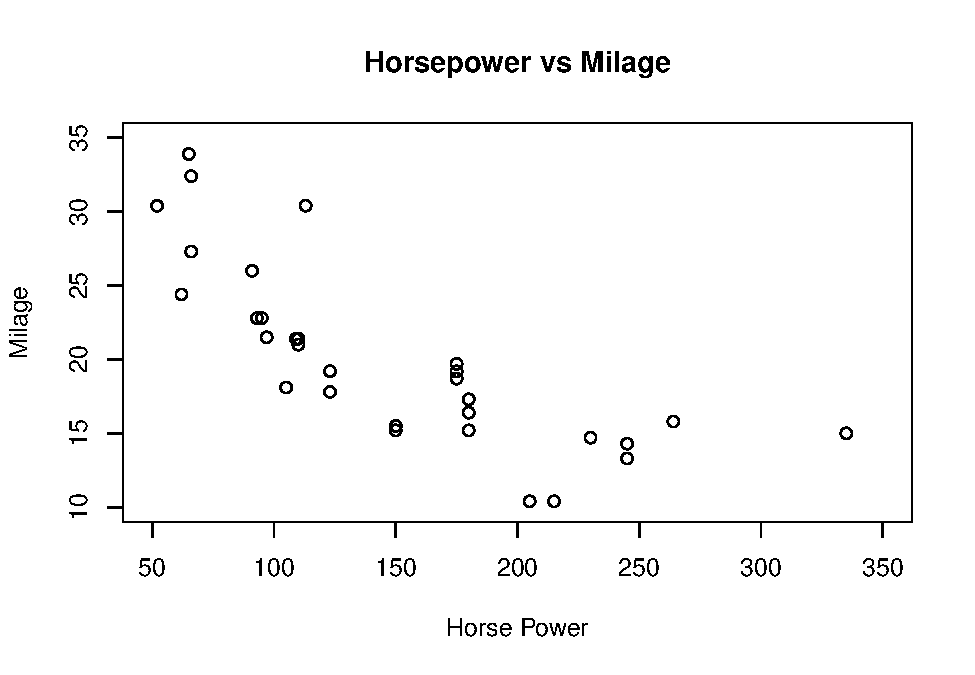
\includegraphics{docs/images/scatter-fig-1.pdf}
\caption{\label{fig:scatter-fig}Grafik Scatter Horse Power dan Milage}
\end{figure}

Istilah
Korelasi : Hubungan anatara suatau variable dengan suatu variable
Regresi : Metode Statistik untuk mencari hubungan antara peubah bebas terhadap peubah tidak bebas
Model regresi : model prediksi yang merupakan hasil regresi
Outlier : data yang nilainya berbeda dari banyak data umumnya atau rata-ratanya.
R kuadrat : Nilai yang menunjukkan porsi pengaruh variable independent terhadap variable dependen
Adjusted R square : Nikalia R kuadrat yang sudah di sesuaikan
Goodness of fit : Dalam Bahasa Indonesia keseuaian model ini menunjukkan model dari regresi yang sudah sesuai
Scatter Diagram: diagram pencar adalah titik yang menghubungkan antara variabel bebas dan varaibel tidak bebas

\hypertarget{latihan-1}{%
\section*{Latihan}\label{latihan-1}}
\addcontentsline{toc}{section}{Latihan}

B-S Pada regresi berganda yang menjadi variable independent boleh lebih dari satu sedangkan variabel dependen hanya satu saja.
B-S Pada regresi variable dependen boeh saja menggunakan variable dummy dan variable gabungan yang lainnya
B-S Regresi dapat menunjukkan kekuatan dalam satu variable independent terhadap variable dependen
B-S Data outlier adalah data yang berbeda dengan lainnya dan menyebabakan kerusakan dalam regresi.
B-S Uji t untuk menunjukkan hubungan yang signifikan variable dependen terhadap variable independent
B-S untuk melihat apakah regresi tersebut sudah baik kita dapat melihat nilai Chi Square
B-S Autokorelasi bias terjadi dalam regresi linier berganda dan dapat menyebabkan kesalahan
B-S Kalau kita menggunakan vairabel dummy adalah variable yang digunakan untuk membedakan antara varabel yang mempunyai kategori.
B-S Nilai Adjusted R Square selalu lebih besar daripada nilai R Square karena ada tambahan berupa penyesuaian nilai banyaknya variable.

Soal
1. Buatlah model dengan cara menilai kesehatan tulang untuk yang segar dengan orang yang sakit sehingga bisa mengembangkan dengan bisa membedakan yang berolahraga ataupun yang tidak?

\begin{enumerate}
\def\labelenumi{\arabic{enumi}.}
\setcounter{enumi}{1}
\item
  Asumsi apakah yang harus dipenuhi dalam regresi logistik coba jelaskan hal itu?
\item
  Pada Altman Z Score setidaknya Z Score dibagi menjadi dua dan ada wilayah abu. saya akan gabungkan wilayah abu ke dalam wilayah yang bangkrut. Akankah ini dibenarkan ? Bagaimana cara menjelaskannya?
\item
  Dalam asumsi ternyata tidak ditemukan maka yang sesuai goodnes of fit atau kebaikan model. Bagaimana mengatasi hal tersebut?
\item
  Kalau di regresi logit maka iti kita lihat kalau kita melihat ada yang berbeda maka itu seperti variabel dikotomi maka akan bisa melihat misalnya dikotomi dari kesehatan jantung untuk satu dan kesehatan lainnya?
\item
  Pada suatu hasil regresi ditunjukkan nilai R squarenya adalah 75\%. Carilah nilai Adjusted R square model tersebut jika jumlah sample 30 dan variable bebasnya ada tiga?
\item
  Carilah contoh beberapa variable independent yang mempengaruhi kepuasan pelanggan?
\item
  Sebutkan beberapa kemungkinan yang ada dari regresi berganda?
\item
  Apakah semakin banyak variable independent akan meningkatkan nilai R Square. Coba jelaskan jawaban anda?
\item
  Apakah beda korelasi dengan regresi?
\end{enumerate}

\hypertarget{regresi-dengan-menggunakan-data-panel}{%
\section{Regresi dengan menggunakan Data Panel}\label{regresi-dengan-menggunakan-data-panel}}

Mengelola data panel di RStudio untuk mengestimasi persamaan regresi dan mencari pengaruh variable independent terhadapa variable dependen.
Salah satu metode untuk mencari pengarih variable adalah dengan data panel. Pengaruh seperti ini adalah untuk kita dapat mengestimasi daripada variable dependen. Data panel adalah data kumpulan dalam bentuk

\hypertarget{membuat-struktur-data-panel}{%
\subsection{Membuat Struktur Data Panel}\label{membuat-struktur-data-panel}}

Rstudio berbeda dari perangkat lunak (software) statistik lainnya. Untuk mengelola dalam analisis appaun membutuhkan struktur data dalam bentuk rstudio. Kalau software lain cukup menyalin dan menempel (copy and paste) data spreadsheet baik itu Excel atau Google Spreadsheet dan langsung dapat untuk mengelola data namun untuk RStuido harus merubahkan dalam bentuk model data yang dikenal oleh Rstudio.
Langkahnya adalah mengimpor file speadhheet dan membuat ebberapa pengaturan yang relative mudah untuk membuat data anda mudah diolah. Khusus untuk analisis panel maka yang dibutuhkan bentuk data atau struktur dari data pdata.frame yang merupakan singkatan panel data frame. Ini berbeda dengan data frame biasa di rtsuido karena ini mempertimbangkan dimensi individual dan juga dimensi waktu. Perlakukan inilah yang membuat berbeda.
Disebelak kana anda dapat mengklik import data set dan pilihlah excel. Ada beberapa pilihan lain seperti spss sas, stata, text dan lain-lain. KAlau mempunyai speadsheet maka pilihlah excel.
Setelah itu anda akan mmeilih beberapa sheet. Kalau anda bekerja dalam banyak sheet di satu file maka anda harus memilih salah satu sheet. Dibawah itu anda pilih. Maka anda harus meperhatikan kerapihan dari text yang anda buat. Misalnya ada sela diantara judul table dan juga isi data maka di table yang kosong itu akan tertulis NA atau Not Available yang berarti data tidak tersedia.
Menyiapkan excel sebagai data
Untuk menyusun data maka yang bisa kita lakukan adalah dengan data. Karena data dnegan speadhseet kita lebih mudah. Kita bisa menyusun dengan data seperti contoh dibawah ini

\begin{Shaded}
\begin{Highlighting}[]
\NormalTok{tobinq }\OtherTok{\textless{}{-}} \FunctionTok{read.csv2}\NormalTok{(}\StringTok{"\textasciitilde{}/jurnal/tobinq3.csv"}\NormalTok{)}
\CommentTok{\#setelah data diupload saya akan membuat data frame khusus panel yang disebut pdata frame dengan seperti ini. jangan lupa gunakan library plm}
\FunctionTok{library}\NormalTok{(plm)}
\end{Highlighting}
\end{Shaded}

\begin{verbatim}
## Warning: package 'plm' was built under R version 4.3.3
\end{verbatim}

\begin{Shaded}
\begin{Highlighting}[]
\NormalTok{ptobinq}\OtherTok{=}\FunctionTok{pdata.frame}\NormalTok{(tobinq,}\AttributeTok{index=}\FunctionTok{c}\NormalTok{(}\StringTok{"Comp"}\NormalTok{,}\StringTok{"Tahun"}\NormalTok{),}\AttributeTok{drop.index =} \ConstantTok{TRUE}\NormalTok{,}\AttributeTok{row.names=}\ConstantTok{TRUE}\NormalTok{)}
\end{Highlighting}
\end{Shaded}

Setelah data sudah benar masuk kita dapat mengecek struktur dari data tersebut

\begin{Shaded}
\begin{Highlighting}[]
\FunctionTok{str}\NormalTok{(ptobinq)}
\end{Highlighting}
\end{Shaded}

\begin{verbatim}
## Classes 'pdata.frame' and 'data.frame':  40 obs. of  3 variables:
##  $ DAR    : 'pseries' Named num  0.49 0.44 0.42 0.4 0.4 0.49 0.44 0.42 0.4 0.4 ...
##   ..- attr(*, "names")= chr [1:40] "Adaro-2014" "Adaro-2015" "Adaro-2016" "Adaro-2017" ...
##   ..- attr(*, "index")=Classes 'pindex' and 'data.frame':    40 obs. of  2 variables:
##   .. ..$ Comp : Factor w/ 8 levels "Adaro","ATPK",..: 1 1 1 1 1 2 2 2 2 2 ...
##   .. ..$ Tahun: Factor w/ 5 levels "2014","2015",..: 1 2 3 4 5 1 2 3 4 5 ...
##  $ DER    : 'pseries' Named num  0.97 0.78 0.72 0.67 0.66 0.97 0.78 0.72 0.67 0.66 ...
##   ..- attr(*, "names")= chr [1:40] "Adaro-2014" "Adaro-2015" "Adaro-2016" "Adaro-2017" ...
##   ..- attr(*, "index")=Classes 'pindex' and 'data.frame':    40 obs. of  2 variables:
##   .. ..$ Comp : Factor w/ 8 levels "Adaro","ATPK",..: 1 1 1 1 1 2 2 2 2 2 ...
##   .. ..$ Tahun: Factor w/ 5 levels "2014","2015",..: 1 2 3 4 5 1 2 3 4 5 ...
##  $ Tobin.Q: 'pseries' Named num  -0.2702 0.2346 0.2706 0.034 0.0336 ...
##   ..- attr(*, "names")= chr [1:40] "Adaro-2014" "Adaro-2015" "Adaro-2016" "Adaro-2017" ...
##   ..- attr(*, "index")=Classes 'pindex' and 'data.frame':    40 obs. of  2 variables:
##   .. ..$ Comp : Factor w/ 8 levels "Adaro","ATPK",..: 1 1 1 1 1 2 2 2 2 2 ...
##   .. ..$ Tahun: Factor w/ 5 levels "2014","2015",..: 1 2 3 4 5 1 2 3 4 5 ...
##  - attr(*, "index")=Classes 'pindex' and 'data.frame':   40 obs. of  2 variables:
##   ..$ Comp : Factor w/ 8 levels "Adaro","ATPK",..: 1 1 1 1 1 2 2 2 2 2 ...
##   ..$ Tahun: Factor w/ 5 levels "2014","2015",..: 1 2 3 4 5 1 2 3 4 5 ...
\end{verbatim}

Sudah benar maka langkahnya adlah mennetukan jenis regresi data panel yang akan kita lakukan. Kemudian sesuai langkah yang sudah kita rencanakan adalah awalnya dengan melakukan regresi dari ketiga metode seperti Pooling (pooling), Fixed Effect (within) dan Random. Dalam contoh kali ini saya akan mennamakan kalau pooling adalah regplmtobinq, untuk fixed effect adalah regplmtobinq2 dan untuk random adalah regplmtobinq3. Dalam tiap perintah aka nada Namanya perintah summary yang artinya adalah menampilkan hasil regresi tersebut.

\begin{Shaded}
\begin{Highlighting}[]
\CommentTok{\#Regresi Model Pooling }
\NormalTok{regplmtobinq}\OtherTok{\textless{}{-}}\FunctionTok{plm}\NormalTok{(Tobin.Q }\SpecialCharTok{\textasciitilde{}}\NormalTok{ DAR}\SpecialCharTok{+}\NormalTok{DER,}\AttributeTok{data=}\NormalTok{ptobinq,}\AttributeTok{model=}\StringTok{"pooling"}\NormalTok{)}

\FunctionTok{summary}\NormalTok{(regplmtobinq)}
\end{Highlighting}
\end{Shaded}

\begin{verbatim}
## Pooling Model
## 
## Call:
## plm(formula = Tobin.Q ~ DAR + DER, data = ptobinq, model = "pooling")
## 
## Balanced Panel: n = 8, T = 5, N = 40
## 
## Residuals:
##     Min.  1st Qu.   Median  3rd Qu.     Max. 
## -1.02749 -0.70659 -0.29490  0.20208  4.38311 
## 
## Coefficients:
##               Estimate Std. Error t-value  Pr(>|t|)    
## (Intercept)  1.5134678  0.3209255  4.7159 3.381e-05 ***
## DAR         -1.7072093  0.4715372 -3.6205 0.0008754 ***
## DER         -0.0038299  0.0682864 -0.0561 0.9555757    
## ---
## Signif. codes:  0 '***' 0.001 '**' 0.01 '*' 0.05 '.' 0.1 ' ' 1
## 
## Total Sum of Squares:    62.653
## Residual Sum of Squares: 46.235
## R-Squared:      0.26204
## Adj. R-Squared: 0.22215
## F-statistic: 6.56918 on 2 and 37 DF, p-value: 0.003619
\end{verbatim}

\begin{Shaded}
\begin{Highlighting}[]
\CommentTok{\#Regresi Model Fixed }
\NormalTok{regplmtobinq2}\OtherTok{\textless{}{-}}\FunctionTok{plm}\NormalTok{(Tobin.Q }\SpecialCharTok{\textasciitilde{}}\NormalTok{ DAR}\SpecialCharTok{+}\NormalTok{DER,}\AttributeTok{data=}\NormalTok{ptobinq,}\AttributeTok{model=}\StringTok{"within"}\NormalTok{)}
\FunctionTok{summary}\NormalTok{(regplmtobinq2)}
\end{Highlighting}
\end{Shaded}

\begin{verbatim}
## Oneway (individual) effect Within Model
## 
## Call:
## plm(formula = Tobin.Q ~ DAR + DER, data = ptobinq, model = "within")
## 
## Balanced Panel: n = 8, T = 5, N = 40
## 
## Residuals:
##      Min.   1st Qu.    Median   3rd Qu.      Max. 
## -1.196028 -0.130457  0.092081  0.186883  1.890241 
## 
## Coefficients:
##      Estimate Std. Error t-value  Pr(>|t|)    
## DAR -2.400988   0.589834 -4.0706 0.0003144 ***
## DER -0.087783   0.042093 -2.0854 0.0456365 *  
## ---
## Signif. codes:  0 '***' 0.001 '**' 0.01 '*' 0.05 '.' 0.1 ' ' 1
## 
## Total Sum of Squares:    17.173
## Residual Sum of Squares: 11.017
## R-Squared:      0.35847
## Adj. R-Squared: 0.16601
## F-statistic: 8.3817 on 2 and 30 DF, p-value: 0.001283
\end{verbatim}

\begin{Shaded}
\begin{Highlighting}[]
\CommentTok{\#Regresi Model Random Effcet}

\NormalTok{regplmtobinq3}\OtherTok{\textless{}{-}}\FunctionTok{plm}\NormalTok{(Tobin.Q }\SpecialCharTok{\textasciitilde{}}\NormalTok{ DAR}\SpecialCharTok{+}\NormalTok{DER,}\AttributeTok{data=}\NormalTok{ptobinq,}\AttributeTok{model=}\StringTok{"random"}\NormalTok{)}
\FunctionTok{summary}\NormalTok{(regplmtobinq3)}
\end{Highlighting}
\end{Shaded}

\begin{verbatim}
## Oneway (individual) effect Random Effect Model 
##    (Swamy-Arora's transformation)
## 
## Call:
## plm(formula = Tobin.Q ~ DAR + DER, data = ptobinq, model = "random")
## 
## Balanced Panel: n = 8, T = 5, N = 40
## 
## Effects:
##                  var std.dev share
## idiosyncratic 0.3672  0.6060   0.4
## individual    0.5506  0.7420   0.6
## theta: 0.6569
## 
## Residuals:
##      Min.   1st Qu.    Median   3rd Qu.      Max. 
## -0.977977 -0.350254 -0.074708  0.106930  2.785480 
## 
## Coefficients:
##              Estimate Std. Error z-value  Pr(>|z|)    
## (Intercept)  1.786432   0.417645  4.2774 1.891e-05 ***
## DAR         -2.087653   0.510836 -4.0867 4.375e-05 ***
## DER         -0.069591   0.043000 -1.6184    0.1056    
## ---
## Signif. codes:  0 '***' 0.001 '**' 0.01 '*' 0.05 '.' 0.1 ' ' 1
## 
## Total Sum of Squares:    22.526
## Residual Sum of Squares: 15.489
## R-Squared:      0.31236
## Adj. R-Squared: 0.27519
## Chisq: 16.8073 on 2 DF, p-value: 0.00022405
\end{verbatim}

\hypertarget{cross}{%
\chapter{Cross-references}\label{cross}}

Cross-references make it easier for your readers to find and link to elements in your book.

\hypertarget{chapters-and-sub-chapters}{%
\section{Chapters and sub-chapters}\label{chapters-and-sub-chapters}}

There are two steps to cross-reference any heading:

\begin{enumerate}
\def\labelenumi{\arabic{enumi}.}
\tightlist
\item
  Label the heading: \texttt{\#\ Hello\ world\ \{\#nice-label\}}.

  \begin{itemize}
  \tightlist
  \item
    Leave the label off if you like the automated heading generated based on your heading title: for example, \texttt{\#\ Hello\ world} = \texttt{\#\ Hello\ world\ \{\#hello-world\}}.
  \item
    To label an un-numbered heading, use: \texttt{\#\ Hello\ world\ \{-\#nice-label\}} or \texttt{\{\#\ Hello\ world\ .unnumbered\}}.
  \end{itemize}
\item
  Next, reference the labeled heading anywhere in the text using \texttt{\textbackslash{}@ref(nice-label)}; for example, please see Chapter \ref{cross}.

  \begin{itemize}
  \tightlist
  \item
    If you prefer text as the link instead of a numbered reference use: \protect\hyperlink{cross}{any text you want can go here}.
  \end{itemize}
\end{enumerate}

\hypertarget{captioned-figures-and-tables}{%
\section{Captioned figures and tables}\label{captioned-figures-and-tables}}

Figures and tables \emph{with captions} can also be cross-referenced from elsewhere in your book using \texttt{\textbackslash{}@ref(fig:chunk-label)} and \texttt{\textbackslash{}@ref(tab:chunk-label)}, respectively.

See Figure \ref{fig:nice-fig}.

\begin{Shaded}
\begin{Highlighting}[]
\FunctionTok{par}\NormalTok{(}\AttributeTok{mar =} \FunctionTok{c}\NormalTok{(}\DecValTok{4}\NormalTok{, }\DecValTok{4}\NormalTok{, .}\DecValTok{1}\NormalTok{, .}\DecValTok{1}\NormalTok{))}
\FunctionTok{plot}\NormalTok{(pressure, }\AttributeTok{type =} \StringTok{\textquotesingle{}b\textquotesingle{}}\NormalTok{, }\AttributeTok{pch =} \DecValTok{19}\NormalTok{)}
\end{Highlighting}
\end{Shaded}

\begin{figure}

{\centering 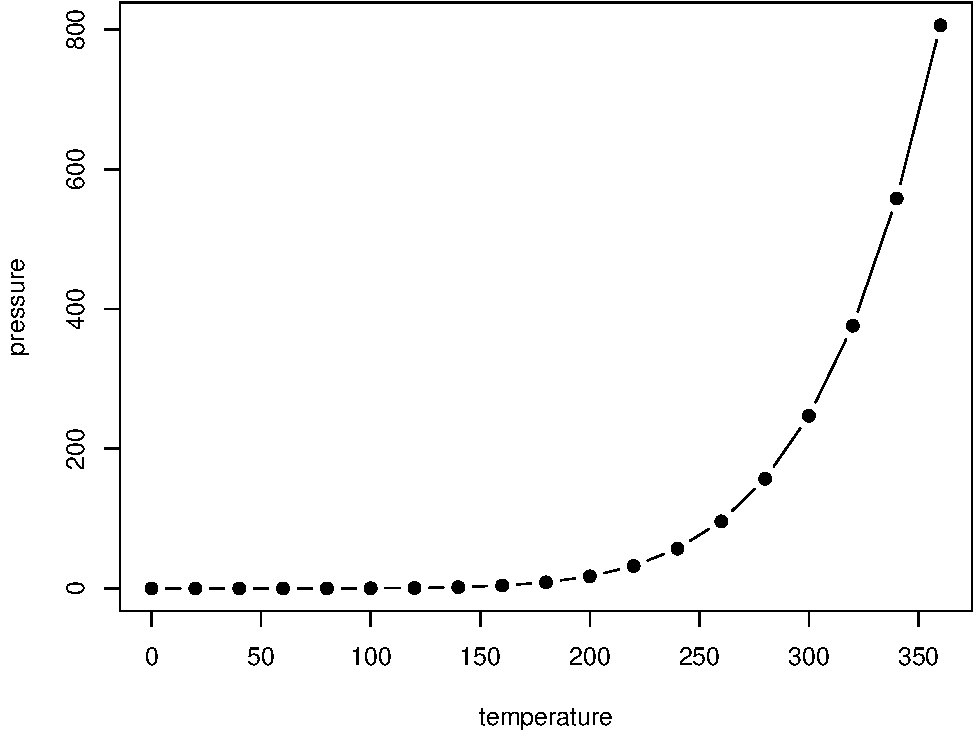
\includegraphics[width=0.8\linewidth]{_main_files/figure-latex/nice-fig-1} 

}

\caption{Here is a nice figure!}\label{fig:nice-fig}
\end{figure}

Don't miss Table \ref{tab:nice-tab}.

\begin{Shaded}
\begin{Highlighting}[]
\NormalTok{knitr}\SpecialCharTok{::}\FunctionTok{kable}\NormalTok{(}
  \FunctionTok{head}\NormalTok{(pressure, }\DecValTok{10}\NormalTok{), }\AttributeTok{caption =} \StringTok{\textquotesingle{}Here is a nice table!\textquotesingle{}}\NormalTok{,}
  \AttributeTok{booktabs =} \ConstantTok{TRUE}
\NormalTok{)}
\end{Highlighting}
\end{Shaded}

\begin{table}

\caption{\label{tab:nice-tab}Here is a nice table!}
\centering
\begin{tabular}[t]{rr}
\toprule
temperature & pressure\\
\midrule
0 & 0.0002\\
20 & 0.0012\\
40 & 0.0060\\
60 & 0.0300\\
80 & 0.0900\\
\addlinespace
100 & 0.2700\\
120 & 0.7500\\
140 & 1.8500\\
160 & 4.2000\\
180 & 8.8000\\
\bottomrule
\end{tabular}
\end{table}

\hypertarget{parts}{%
\chapter{Parts}\label{parts}}

You can add parts to organize one or more book chapters together. Parts can be inserted at the top of an .Rmd file, before the first-level chapter heading in that same file.

Add a numbered part: \texttt{\#\ (PART)\ Act\ one\ \{-\}} (followed by \texttt{\#\ A\ chapter})

Add an unnumbered part: \texttt{\#\ (PART\textbackslash{}*)\ Act\ one\ \{-\}} (followed by \texttt{\#\ A\ chapter})

Add an appendix as a special kind of un-numbered part: \texttt{\#\ (APPENDIX)\ Other\ stuff\ \{-\}} (followed by \texttt{\#\ A\ chapter}). Chapters in an appendix are prepended with letters instead of numbers.

\hypertarget{footnotes-and-citations}{%
\chapter{Footnotes and citations}\label{footnotes-and-citations}}

\hypertarget{footnotes}{%
\section{Footnotes}\label{footnotes}}

Footnotes are put inside the square brackets after a caret \texttt{\^{}{[}{]}}. Like this one \footnote{This is a footnote.}.

\hypertarget{citations}{%
\section{Citations}\label{citations}}

Reference items in your bibliography file(s) using \texttt{@key}.

For example, we are using the \textbf{bookdown} package \citep{R-bookdown} (check out the last code chunk in index.Rmd to see how this citation key was added) in this sample book, which was built on top of R Markdown and \textbf{knitr} \citep{xie2015} (this citation was added manually in an external file book.bib).
Note that the \texttt{.bib} files need to be listed in the index.Rmd with the YAML \texttt{bibliography} key.

The RStudio Visual Markdown Editor can also make it easier to insert citations: \url{https://rstudio.github.io/visual-markdown-editing/\#/citations}

\hypertarget{blocks}{%
\chapter{Blocks}\label{blocks}}

\hypertarget{equations}{%
\section{Equations}\label{equations}}

Here is an equation.

\begin{equation} 
  f\left(k\right) = \binom{n}{k} p^k\left(1-p\right)^{n-k}
  \label{eq:binom}
\end{equation}

You may refer to using \texttt{\textbackslash{}@ref(eq:binom)}, like see Equation \eqref{eq:binom}.

\hypertarget{theorems-and-proofs}{%
\section{Theorems and proofs}\label{theorems-and-proofs}}

Labeled theorems can be referenced in text using \texttt{\textbackslash{}@ref(thm:tri)}, for example, check out this smart theorem \ref{thm:tri}.

\begin{theorem}
\protect\hypertarget{thm:tri}{}\label{thm:tri}For a right triangle, if \(c\) denotes the \emph{length} of the hypotenuse
and \(a\) and \(b\) denote the lengths of the \textbf{other} two sides, we have
\[a^2 + b^2 = c^2\]
\end{theorem}

Read more here \url{https://bookdown.org/yihui/bookdown/markdown-extensions-by-bookdown.html}.

\hypertarget{callout-blocks}{%
\section{Callout blocks}\label{callout-blocks}}

The R Markdown Cookbook provides more help on how to use custom blocks to design your own callouts: \url{https://bookdown.org/yihui/rmarkdown-cookbook/custom-blocks.html}

\hypertarget{asumsi-regresi-linear}{%
\chapter{Asumsi Regresi Linear}\label{asumsi-regresi-linear}}

Setiap metode yang kita apakah harus kita ingat mempunyau syarat dan kondisi. Seperti kita mau membeli suatu maka kita menemukan suatau kondisi yang harus kita penuhi . Tanpa syarat dan kondisi tersebut maka kita tidak akan mendapatkan apa yang kita maui. Ada beberapa gejala kalau tidak bisa dibilang penyakit yang terdapat pada Regresi linear. Hal tersebut harus kita lewati sebagai syarat nilai peramalan dan juga koefisien determinasi dari regresi tersebut benar-benar valid.
Hasil sutau persamaan regresi bisa berbeda satu sama lannya. Ini bukan terjasi kesalahan data karena Namanya data tidak pernah salah selama penegumpulanay sudah benar. Adanya data yang melewati rata-rata atau outlier dapat menyebabkan hal serprti itu. Adanya perbedaan itu maka kita harus memperbaiki terlebih dahulu asumsi. Setiap metode mmepunyai syarat begitu juga regresi harus memenuhi syarat-syarat tersebut.
Ada beberapa hal yang membuat regresi tersebut tidak akan menjadi valid yang bisa kita perhatikan seperti ini:

\hypertarget{multikolinearitas}{%
\section{Multikolinearitas}\label{multikolinearitas}}

Kita mau mencari hubungan antara variabel independen dengan variabel yang dependen, hanya saja terjadi hubungan yang baik antara variabel independen dengan variabel independen juga atau sesama variabel independen. Hubungan ini tidak bisa dibiarkan karena akan menyebabkan variabel tersebut merusak nilai perhitungan dari regresi.
Hubungan sesama variabel independen dapat menyebabkan nilai R kuadrat (R2) begitu tinggi, namun penduga (peramalannya menjadi bias). Untuk itu hal ini harus diatasi dengan cara membuang salah satu variabel yang sama.
Sebenarnya tidak terlalu sulit untuk menduga akan terjadinya multikolinearitas . Ketika kita melihat ada data tabel yang begitu mirip antara sesama variabel independen, kita harus mengecek apakah kita menyalin data yang sama untuk variabel yang berbeda. Terkadang salah satu data merupakan kelipatan dari data yang lainnya dan inilah yang menyebabkan korelasi begitu tinggi. Pastikan juga tidak ada data yang sama masuk ke dalam variable yang berbeda. Jika yakin ternyata data tersebut juga memang benar maka bisa jadi itu data memang mempunyai sifat yang sama. Hubungan antara korelasi keduanya sangat besar sekali hampir sampai lebih dari 80\%. Kalau kita menggunakan Korelasi Pearson maka kita akan mendapatkan nilai korelasi yang tinggi.\\
Kesalahan ini bisa jadi karena memang datanya seperti itu. Seperti harga ayam kampung dengan harga ayam ras maka kita bisa pastikan keduanya mempunyai hubungan yang positif. Kalau harga ayam ras naik maka harga ayam kampung juga naik. Meski keduanya mempunyai harga yang berbeda namun mempunyai peluang untuk naik pada waktu yang sama atau turun pada waktu yang sama.
Untuk mendeteksi dari gejala ini adalah dengan melihat nilai VIF yang ada dalam software statistik. Nilai VIF yang lebih besar dari 10 maka terjadi yang namanya multikolinearitas. Kemudian ada juga nilai eugin value yang lebih dari 0,001.
Untuk mengatasi multikolinearitas adalah tidak sulit. Hanya saja pilihannya adalah membuang salah satu variable dalam regresi multi variable. Hanya saja masalahnya adalah pilihan yang mana yang mau dibuang kadang ini menjadi pilihan yang dilematis.

\hypertarget{autokorelasi}{%
\section{Autokorelasi}\label{autokorelasi}}

Nilai Autokorelasi terjadi ketika deret waktu mempunyai nilai galat (error) yang berkorelasi .Hal ini terjadi karena data berseri (time series) yang ada dalam suatu model. Pada beberapa kasus ternyata data cross section sendiri juga dapat mengalami autokorelasi. Pada autokorelasi terjadi karena galat yang berubah menurut waktu.

Untuk menilai apakah adanya terjadinya korelasi, kita dapat menggunakan kriteria sebagai berikut yakni dl (Durbin lower) yang berarati nilai Durbin terendah atau du (Durbin upper) yang berarti nilai durbin di atas. Semua nilai yang berada di antara kedua nilai tersebut harus memenuhi syarat sehingga, model yang kita buat sudah dikatakan terbebas dari autokorelasi.

Autokorelasi adalah suatu hubungan galat atau error yang berhubungan. Hubungan tersebut akan semakin membesar dan semakin mengecil pada tingkat peramalan yang dibuat oleh model yang memiliki gejala autokorelasi. Mau tidak mau nilai dari autokorelasi harus dihilangkan terlebih dahulu. Dengan kata lain kita harus membuat sesuatu model yang terbebas dari autokorelasi. Apapun regresi yang terjadi kesalahan termasuk autokrelasi karena adanya data tersebut. Karenanya pastikan terlebih dahulu data yang anda kumpulkan tersebut memang sudah benar. Setelah yakin kalau sudah melakukan regresi lagi.

Untuk mendeteksi gejala ini kita mengamati pola residual terhadap urutannya atau t. Kalau data residual mempunyai pola tertentu baik meningkat maupun menurun maka patut dicurigai terjadinya autokorelasi. Kalau data tidak mempunyai pola (pattern) atau data tersebar dengan bebas maka tidak terjadi autokorelasi.

Selain melakukan uji Durbin Watson kita bsia melakukan uji yang lain seperti Ljung Box uji ini juga dapat untuk menduga regresi yang kita lakukan. Uji ini akan menempatkan H0 atau Hipotesis nol adalah hasil regresi terdapat mengandung autokorelasi sedangkan hipotesis alternatif (Ha) menunjukkan kalau tidak ada autokorelasi dalam model yang diuji.

Nilai Durbin Watson yang dikembangkan mempunyai rumus seperti di bawah ini:

du= (∑\emph{(t=1)\^{}n▒(e}(t-1)-e\_t )\^{}2 )/(e\_t\^{}2 )

Dengan et = nilai error ke t
et-1 = nilai error ke t-1

Dalam uji ini ditetapkan sebagai Hipotesis nol adalah jika terjadi autokorelasi sedangkan Ha diterima jika terjadi autokorelasi

H0 : ρ = 0 tidak terjadi autokrelasi
Ha : ρ ≠ 0 terjadi autokorelasi

Autokorelasi itu terjadi karena danya kandungan data series tetapi seperti disinggung diatas kalau data cross section pun juga menjadi autokorelasi untuk mengatasi adalah kita bisa melakukan hal seperti ini. Kita menggunakan differencing pada data time series. Setelah difference atau pembedaan ada kemungkinan data time series juga bisa diperbaiki.

Salah satu mengatasi dengan menggunakan lag. Lag ini adalah konsekuensi dengan nilai dari regresi tersebut. Ada beberapa variable respon tidak selalu merespon dengan cepat. Karenanya ada sebuah respon tersebut maka aka nada repson yang terlambat sekali . Adapun bentuk antisipasi memang semuanya bervariasi karena memang tidak langsung. Bahkan kita curiga kalau suatu reaksi sudah diketahui sebelumnya berarti ada efek antisipasi oleh respon tersebut.

\hypertarget{heteroskedatisitas}{%
\section{Heteroskedatisitas}\label{heteroskedatisitas}}

Pada mengumpulkan data, kita mungkin kurang memperhatikan adanya variance yang berbeda. Seharusnya dalam peramalan regresi juga kita harus memperhatikan asumsi bahwa error tidak berbeda E( ε ) = 0. Adanya perbedaan karena memang sulit sekali bagi regresi linear untuk mencari nilai yang paling mendekati dengan garis persamaan regresi yang mendekati dari data tersebut.

Hal ini harus segera dipebaiki. Sebelum kita melihat adanya dugaan heteroskedatisitas kita harus melihat terlebih dahulu adanya potensi dari heteroskedatisitas. Kita tahu adanya variance yang berbeda anatara Y prediksi. Tentu untuk meminimalkan kita bisa menghilangkan hal tersebut. Penyebab dari terjadinya heteroskeditas adalah nilai yang ekstrim atau outlier dalam data. Maka data outlier tersebut jauh dari peramalan sedangkan kita sulit untuk membuat ramalan yang tepat.

Di awal mungkin kita tidak bisa untuk menebak atau menduga apakah yang terjadi dalam regresi kita tetapi kita bisa lakukan antara lain

\begin{verbatim}
Plot scatter antara predictor value dan residual kalau memuat grafik seperti pola topi runcing atau cone, maka akan adanya heteroskedatisitas 
Plot scatter antara nilai yang diprediksi dan residual kalau berbentuk seperti pola tertentu bisa jadi pola sebaran itu seperti ada garis yang mempunyai trend cenderung ke atas atau ke bawah. Ada sekumpulan garis residual yang membentuk suatu pola. Tentu hal ini tidak baik karena menunjukkan adanya pola tertentu. 
Breusch pagan dan white test adalah untuk mendeteksi adanya heterosskedatisitas dengan cara menghitung ??
\end{verbatim}

Setelah kita mengetahui adanya gejala heteroskedatisitas maka kita harus memperbaiki hal tersebut. Ada beberapa hal namun sebelum kita memperbaiki kita harus melihat dulu mengapa terjadi heteroskedatistas

Hetereoskedatisitas mengakibatkan peramalan menjdi bias membuat estimasi tidak efisien. Dalam regresi heteroskedatisitas mengakibatkan nilai t akan besar sehingga seolah terlihat nilai yang sangat signifikan. Nilai tersebut tentu tidak baik dan tidak mencerminkan nilai yang sesungguhnya. Supranto

Ibarat memperbaiki Kursi
Ketika kita memperbaiki suatu gejala contoh autokorelasi bisa jadi heteroskedatisitas yang tadinya belum ada akan muncul. Hal ini bisa terjadi kalau perbaikan pada kita seperti kita memukul kayu di suatu tempat maka akan ada yang terpukul di lain pihak hal itu biasa saja dalam praktik untuk membuat suatu model yang tepat . Maunya kita membetulkan satu namun tidak merusak yang lain tapi itu tidak bisa terjadi. Kalau kita mengetahui akar masalahnya maka kita akan bisa menyelesaikan masalahnya.

Terkadang beberapa hal yang banyak yang sudah kita laakukan namun belum memasukkan atau belum menemukan suatu model yang sudah terbebas dari keseluruhan asumsi normal yang menjadi syarat dalam regresi sudah terbebas. Baru model tersebut dapat dikatakan menjadi estimator atau penduga yang baik.

Untuk itu memang perlu kesabaran dari proses pengolahan data tersebut. Karena adalah hal yang ketentuan bisa menjadi berubah maka hal itu harus melewati revisi juga.

Regresi linier sederhana Regresi linier bergabda
Asumsi Normal V V
Multikolinearitas X V
Heteroskedatiositas V V
Autokorelasi V V

\hypertarget{asumsi-normalitas}{%
\section{Asumsi Normalitas}\label{asumsi-normalitas}}

Kembali lagi ke dalam statistik dasar kalau kita tahu bahwa regresi tersebut juga memiliki data yang normal atau normalitas. Nilai residual dari peramalan tersebut terdistribusi normal. Jadi bukan datanya yang terdistribusi normal. Ketika hasil regresi linier berganda ini adalah kita akan melihat nilai residual adalah normal atau terdistribusi normal. Data yang normal adalah data yang tersebar menurut seperti lonceng tersebut. Data yang tidak tersebar normal berarti ada sesuatu yang tidak sesuai. Karenannya hasil prediksi dari data tidak normal menjadi tidak konssten.

Untuk membuktikan kalau sebuah hasil residual terdistribusi normal maka kita bisa melihat dari tabel satu grafik batang yang menunjukkan sebaran yang normal. Sebaran normal seperti bentuk gunung yang simetris atau lonceng yang simetris. Baik sisi Kanan dan kiri mempunyai dua sisi yang terbagi sempurna. Kalau sudah seperti ini mska data akn tersebar normal. Pada dasarnya kita sulit sekali mendapatkan sesuatu yang normal. Terkadang dan memang seringnya muncul grafik yang tidak normal. Hal ini biasa saja karena persebaran data tersebut sering tidak normal apalagi kalau menggunakan data yang dalam jumlah terbaras. Ada kemungkinan data akan mempunyai banyak outlier yang akan menyebabkan residual malah tidak baik model permalannya

Kalau ada bagian grafik yang cukup meragunakan maka kita bisa menjalankan uji Run atau Runs Test . Uji ini adalah uji non parametrik yang dapat menguji run atau giliran dari data residual tersebut. Adapun uji run mempunyai hipotesis seerti ini
Ho: Data terdistribusi normal
H1 : Data tidak terdistribusi normal

JIka hasil uji run menunjukkan nilai peluang (probability value) lebih besar 0,05 maka hipotesis nol (Ho) diterima maka data terdistribusi normal. Sebaliknya jika nilai peluan \textless0,05 maka ada indikasi residual data tersebut tersebar dengan tidak normal. Maka kita menolak Ho dan menerima H1.
Selain run kita juga data melakukan ujia Shapiro Wilk

  \bibliography{book.bib,packages.bib}

\end{document}
